\documentclass[border=18pt]{standalone}
\usepackage[T1]{fontenc}
\usepackage{lmodern,amsmath,amssymb}
\hyphenpenalty=10000
\exhyphenpenalty=10000
\usepackage{tikz}
\usetikzlibrary{arrows.meta,calc}
\definecolor{ink}{HTML}{49372F}
\definecolor{copper}{HTML}{AE6540}
\definecolor{ivory}{HTML}{FFF9F1}
\definecolor{gold}{HTML}{B88D54}
\begin{document}
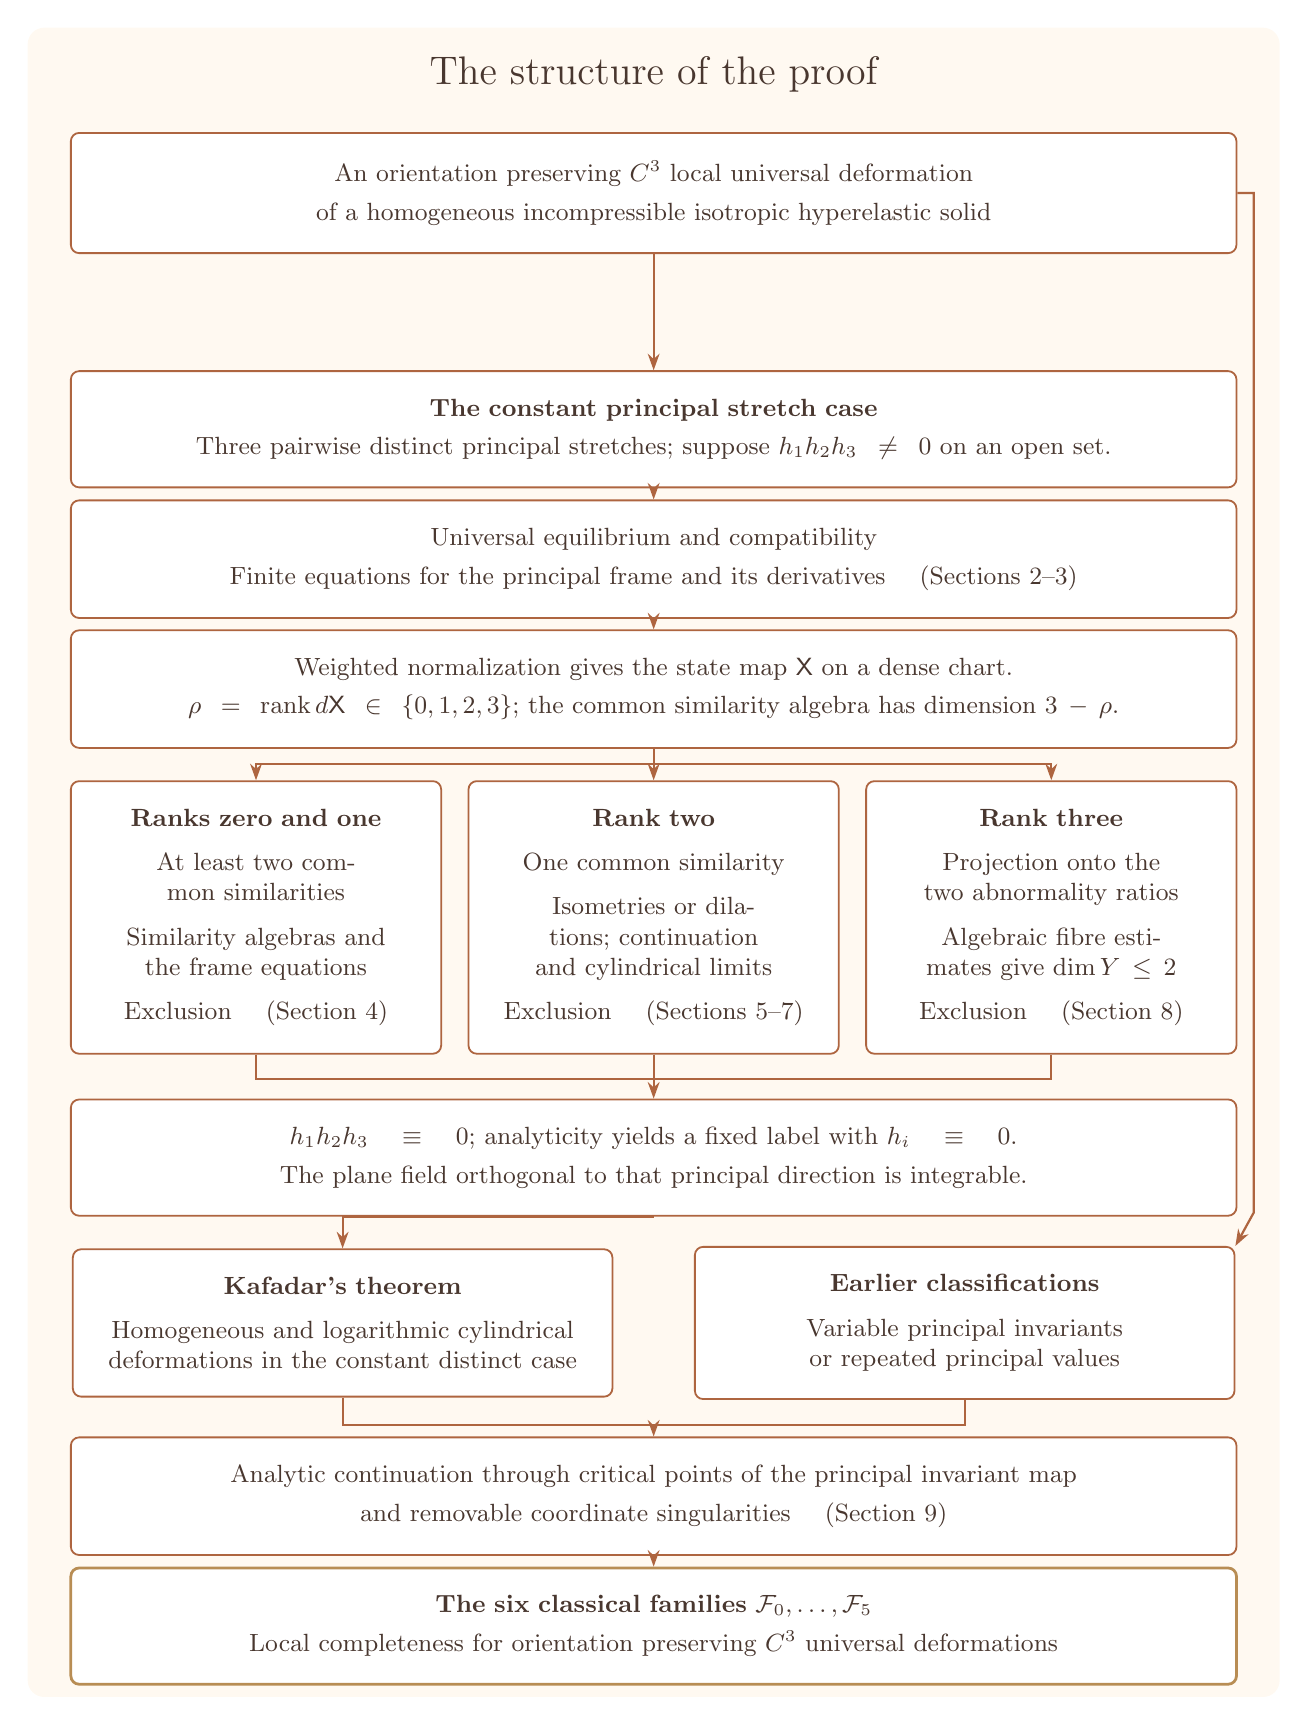
\begin{tikzpicture}[
  font=\small, text=ink,
  box/.style={draw=copper,line width=.65pt,rounded corners=3pt,
    fill=white,align=center,inner sep=10pt},
  wide/.style={box,text width=14.1cm,minimum height=1.05cm},
  branch/.style={box,text width=4.0cm,minimum height=3.0cm},
  half/.style={box,text width=6.15cm,minimum height=1.55cm},
  arrow/.style={-{Stealth[length=2.1mm,width=1.5mm]},draw=copper,line width=.8pt},
  pathline/.style={draw=copper,line width=.8pt}
]
\fill[ivory,rounded corners=6pt] (-7.95,4.2) rectangle (7.95,-17.0);
\node[font=\Large] at (0,3.6) {The structure of the proof};
\node[wide] (universal) at (0,2.1) {
  An orientation preserving $C^3$ local universal deformation\\[3pt]
  of a homogeneous incompressible isotropic hyperelastic solid
};
\node[wide] (input) at (0,-.9) {
  \textbf{The constant principal stretch case}\\[3pt]
  Three pairwise distinct principal stretches; suppose $h_1h_2h_3\ne0$ on an open set.
};
\node[wide] (frame) at (0,-2.55) {
  Universal equilibrium and compatibility\\[3pt]
  Finite equations for the principal frame and its derivatives \quad (Sections 2--3)
};
\draw[arrow] (universal.south)--(input.north);
\node[wide] (state) at (0,-4.2) {
  Weighted normalization gives the state map $\mathsf X$ on a dense chart.\\[3pt]
  $\rho=\operatorname{rank}d\mathsf X\in\{0,1,2,3\}$; the common similarity algebra has dimension $3-\rho$.
};
\draw[arrow] (input.south)--(frame.north);
\draw[arrow] (frame.south)--(state.north);
\node[branch] (low) at (-5.05,-7.1) {
  \textbf{Ranks zero and one}\\[5pt]
  At least two common similarities\\[5pt]
  Similarity algebras and the frame equations\\[5pt]
  Exclusion \quad (Section 4)
};
\node[branch] (two) at (0,-7.1) {
  \textbf{Rank two}\\[5pt]
  One common similarity\\[5pt]
  Isometries or dilations; continuation and cylindrical limits\\[5pt]
  Exclusion \quad (Sections 5--7)
};
\node[branch] (three) at (5.05,-7.1) {
  \textbf{Rank three}\\[5pt]
  Projection onto the two abnormality ratios\\[5pt]
  Algebraic fibre estimates give $\dim Y\le2$\\[5pt]
  Exclusion \quad (Section 8)
};
\coordinate (fork) at (0,-5.15);
\draw[pathline] (state.south)--(fork);
\draw[arrow] (fork)-| (low.north);
\draw[arrow] (fork)--(two.north);
\draw[arrow] (fork)-| (three.north);
\node[wide] (integrable) at (0,-10.15) {
  $h_1h_2h_3\equiv0$; analyticity yields a fixed label with $h_i\equiv0$.\\[3pt]
  The plane field orthogonal to that principal direction is integrable.
};
\coordinate (merge) at (0,-9.15);
\draw[pathline] (low.south)|-(merge);
\draw[pathline] (two.south)--(merge);
\draw[pathline] (three.south)|-(merge);
\draw[arrow] (merge)--(integrable.north);
\node[half] (kafadar) at (-3.95,-12.25) {
  \textbf{Kafadar's theorem}\\[5pt]
  Homogeneous and logarithmic cylindrical deformations in the constant distinct case
};
\node[half] (classical) at (3.95,-12.25) {
  \textbf{Earlier classifications}\\[5pt]
  Variable principal invariants or repeated principal values
};
\draw[arrow] (integrable.south) -| (kafadar.north);
\draw[arrow] (universal.east)--(7.62,2.1)--(7.62,-10.85)--(classical.north east);
\node[wide] (continuation) at (0,-14.45) {
  Analytic continuation through critical points of the principal invariant map\\[3pt]
  and removable coordinate singularities \quad (Section 9)
};
\coordinate (join) at (0,-13.55);
\draw[pathline] (kafadar.south)|-(join);
\draw[pathline] (classical.south)|-(join);
\draw[arrow] (join)--(continuation.north);
\node[wide,draw=gold,line width=1pt] (result) at (0,-16.1) {
  \textbf{The six classical families $\mathcal F_0,\ldots,\mathcal F_5$}\\[3pt]
  Local completeness for orientation preserving $C^3$ universal deformations
};
\draw[arrow] (continuation.south)--(result.north);
\end{tikzpicture}
\end{document}
